\documentclass[a4paper,12pt]{article}

% Import the deliverable package from common directory
\usepackage{../common/deliverable}

% Tell LaTeX where to find graphics files
\graphicspath{{../common/logos/}{./figures/}{../}}

\usepackage{xspace}
\usepackage{subcaption}
\usepackage{placeins}
\usepackage{tikz}
\usetikzlibrary{positioning,fit,arrows.meta}

% Include a screenshot if present in ./figures/, otherwise render a framed
% placeholder so the document always compiles while screenshots are collected.
\newcommand{\figureOrPlaceholder}[2]{%
  \IfFileExists{./figures/#1}{\includegraphics[width=400pt]{#1}}{%
    \fbox{\parbox[c][5cm][c]{380pt}{\centering\itshape Screenshot to be added:\\ #2\\ (\texttt{figures/#1})}}}}

% Set the deliverable number (without the D prefix, it's added automatically)
\setdeliverableNumber{2.7}

% Begin document
\begin{document}

% Create the title page with the title as argument
\maketitlepage{Deployment of the PoC platform}

\newpage

% Main Table using the new environment and command
\begin{deliverableTable}
    \tableEntry{Deliverable title}{D2.7: Deployment of the PoC platform}
    \tableEntry{Deliverable number}{D2.7}
    \tableEntry{Deliverable version}{0.1}
    \tableEntry{Date of delivery}{31/07/2026}
    \tableEntry{Actual date of delivery}{[TBD]}
    \tableEntry{Nature of deliverable}{Report}
    \tableEntry{Dissemination level}{Public}
    \tableEntry{Work Package}{WP2}
    \tableEntry{Partner responsible}{eXact lab}
\end{deliverableTable}

% Abstract and Keywords Section
\begin{deliverableTable}
    \tableEntry{Abstract}{ dealii-X D2.7 reports on the deployment of the
        first version of the Proof of Concept (PoC) platform, whose design was
        presented in D2.6. The platform, named DealiiX Platform, is accessed through a desktop
        application which provides a node-based low-code editor for building
        computational graphs, which are then executed by CORAL, a C++ computational
        graph engine backed by the deal.II library. The no-code layer
        envisioned in D2.6 is realized through subnetwork nodes, allowing users
        to encapsulate low-code graphs into reusable high-level components.
        The platform transparently targets computational resources ranging
        from the local machine to remote HPC systems managed by the Slurm
        scheduler, including MPI-parallel executions, and integrates a
        collaborative project server and a visualization service. This
        deliverable describes the architecture and the main features of the
        deployed platform, its packaging, testing and continuous integration
        infrastructure, and outlines the activities planned for the final
        development phase of the project. }
        \tableEntry{Keywords}{
            PoC platform;
            low-code interface;
            no-code interface;
            computational graph;
            CORAL;
            deal.II;
            metascheduler;
            HPC
        }
\end{deliverableTable}

\newpage

\begin{documentControl}
  \addVersion{0.1}{16/07/2026}{M. Franzon}{Initial draft}
  \addVersion{0.2}{29/07/2026}{P. Colturi, M. Franzon}{Added the section on
    testing with the lighthouse applications and early-user feedback; revised
    the description of the HPC deployment and of the planned orchestration
    layer; updated the Outlook}
\end{documentControl}

\subsection*{{Approval Details}}
Approved by: [TBD] \\
Approval Date: [TBD]

\subsection*{{Distribution List}}
\begin{itemize}
    \item [] - Project Coordinators (PCs)
    \item [] - Work Package Leaders (WPLs)
    \item [] - Steering Committee (SC)
    \item [] - European Commission (EC)
\end{itemize}

\vspace*{2cm}

\disclaimer

\newpage

\tableofcontents % Automatically generated and hyperlinked Table of Contents

\newpage


\section{\textcolor{EUblue}{Introduction}}

Deliverable D2.6 presented the design of the Proof of Concept (PoC) platform
of the dealii-X project: a single environment in which professionals with
different levels of technical expertise can build, run and inspect
simulations based on the dealii-X libraries, without having to deal with the
complexity of the traditional HPC workflow. The design identified four main
requirements: a collaborative space, a modular architecture, an interaction
model that allows deep customization without requiring specific coding
skills, and a transparent usage of computational resources, from local
machines to HPC clusters. These requirements led to the adoption of a
combined low-code/no-code approach, in which users can define custom no-code
nodes in terms of low-code logic.

The present deliverable reports on the deployment of the first version of
the PoC platform, named \emph{DealiiX Platform}. Following the development
plan outlined in D2.6, the implementation activities of tasks 2.6.2
(development of the no-code/low-code graphical user interface) and 2.6.3
(development of a meta-scheduler system) started in M7 and proceeded
iteratively, with a first version of the platform available at M17 and the
deployment and testing phase (task 2.6.4) carried out between M18 and M22.
The platform has been developed in the open, with an iterative release
process: six versions have been released between M12 and M22, each
accompanied by a public changelog, packaged installers for Linux and macOS,
and an automated test suite.

The rest of the deliverable is organized as follows. Section 2 presents the
architecture of the platform and its components. Section 3 describes the
low-code node editor, the concrete realization of the design sketched in
section 2 of D2.6. Section 4 describes the no-code layer, based on
subnetwork nodes. Section 5 covers the execution modes and the
meta-scheduling functionality, which transparently target local and remote
computational resources. Section 6 presents the collaborative and
visualization services. Section 7 reports on the testing of the platform
with the dealii-X lighthouse applications and on the feedback collected
during the deployment phase. Section 8 reports on packaging, deployment and
quality assurance, and section 9 outlines the activities planned for the
final phase of the project.

\section{\textcolor{EUblue}{Architecture of the PoC platform}}

The PoC platform is composed of four cooperating components, shown in
Fig.~\ref{architecture}:

\begin{itemize}
    \item \textbf{DealiiX Platform}, the desktop application that provides
        the user interface. It is built with the Electron framework and the
        Svelte~5 web framework, and embeds the node-based canvas editor on
        which the low-code and no-code interactions take place.
    \item \textbf{CORAL} (Computational Object-oriented Representation And
        Library), the C++ computational graph engine that executes the
        graphs built in the editor. CORAL exposes the classes and functions
        of an underlying scientific library as a \emph{registry} of nodes,
        and executes \emph{networks} of such nodes. The main backend is a
        deal.II plugin, which makes the deal.II finite element machinery
        available as graph nodes.
    \item \textbf{Coral Remote Server}, a REST API server written in Go
        that provides user authentication and collaborative project
        management, backed by an SQLite database.
    \item \textbf{Coral Visualizer}, a Python web application for the
        visualization of simulation results in VTK formats, built on the
        Trame framework with a ParaView-based rendering backend.
\end{itemize}

\begin{figure}
    \centering
    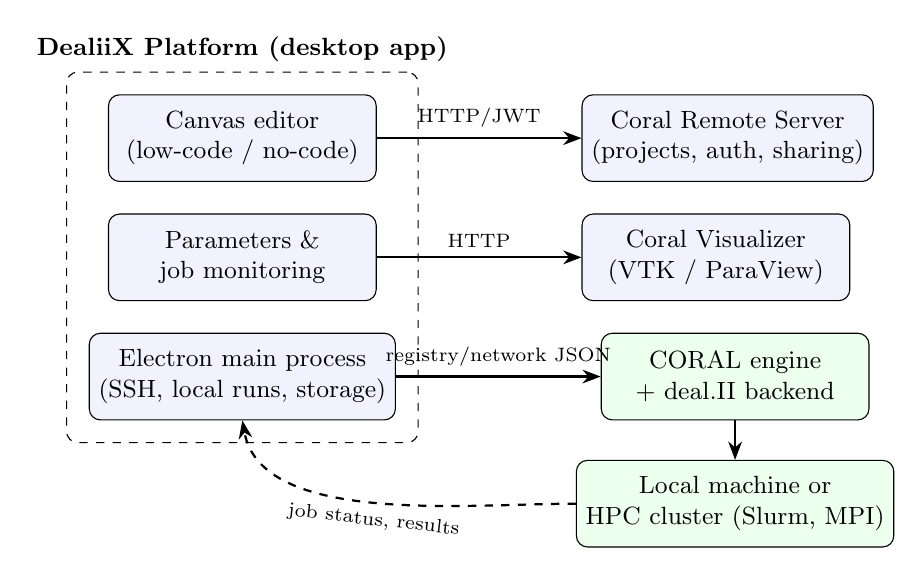
\begin{tikzpicture}[
        font=\small,
        box/.style={draw, rounded corners, align=center, fill=blue!5,
            minimum width=3.4cm, minimum height=1.1cm},
        group/.style={draw, rounded corners, dashed, inner sep=8pt},
        arr/.style={-{Stealth}, thick},
    ]
        % Desktop app
        \node[box] (canvas) {Canvas editor\\ (low-code / no-code)};
        \node[box, below=0.4cm of canvas] (params) {Parameters \&\\ job monitoring};
        \node[box, below=0.4cm of params] (main) {Electron main process\\ (SSH, local runs, storage)};
        \node[group, fit=(canvas)(params)(main), label={[anchor=south]above:\textbf{DealiiX Platform (desktop app)}}] (app) {};

        % Right column: services
        \node[box, right=2.6cm of canvas] (server) {Coral Remote Server\\ (projects, auth, sharing)};
        \node[box, right=2.6cm of params] (viz) {Coral Visualizer\\ (VTK / ParaView)};

        % Bottom right: execution
        \node[box, right=2.6cm of main, fill=green!7] (coral) {CORAL engine\\ + deal.II backend};
        \node[box, below=0.5cm of coral, fill=green!7] (hpc) {Local machine or\\ HPC cluster (Slurm, MPI)};

        \draw[arr] (canvas.east) -- node[above, sloped, font=\scriptsize]{HTTP/JWT} (server.west);
        \draw[arr] (params.east) -- node[above, sloped, font=\scriptsize]{HTTP} (viz.west);
        \draw[arr] (main.east) -- node[above, sloped, font=\scriptsize]{registry/network JSON} (coral.west);
        \draw[arr] (coral) -- (hpc);
        \draw[arr, dashed] (hpc.west) to[out=180, in=-80, looseness=0.8]
            node[below, sloped, font=\scriptsize]{job status, results} (main.south);
    \end{tikzpicture}
    \caption{Architecture of the PoC platform and its components}
    \label{architecture}
\end{figure}

The desktop application and CORAL communicate through two JSON-based
protocols, which constitute the contract between the user interface and the
computational engine:

\begin{itemize}
    \item The \textbf{registry protocol} describes the node types made
        available by a CORAL backend: for each node, its arguments with
        their types, its input and output connections, and its nature
        (constructor, member function, free function, etc.). The registry is
        loaded by the application at startup, validated, and used to
        populate the palette of available nodes.
    \item The \textbf{network protocol} describes a computational graph as a
        list of nodes and typed edges. It is used to save and load projects,
        to exchange graphs between users, and to submit graphs to CORAL for
        execution.
\end{itemize}

This clean separation keeps the user interface completely agnostic of the
underlying simulation library: any library wrapped by a CORAL backend
automatically becomes available in the visual editor, without changes to the
application. This fulfills one of the key modularity requirements set in
D2.6.

\section{\textcolor{EUblue}{The low-code node editor}}
\label{sec:lowcode}

The low-code interface implements the node-based programming model designed
in section 2 of D2.6. The minimal set of object-oriented entities identified
there is mapped onto a family of node types: elementary constructors for
primitive values (integers, floating point numbers, booleans, strings),
class constructors, member functions (including \texttt{const} and
value-returning methods), free functions, and abstract base classes used for
polymorphic connections. Each node exposes typed input and output pins, and
edges between pins are validated in real time against the type system: a
connection is accepted only if the output type of the source node matches
the input type of the target node, including inheritance relations through
abstract base classes. The same validation is applied when a graph is
imported from a file or loaded from the remote server, so that only
well-formed graphs reach the execution engine.

\begin{figure}
    \centering
    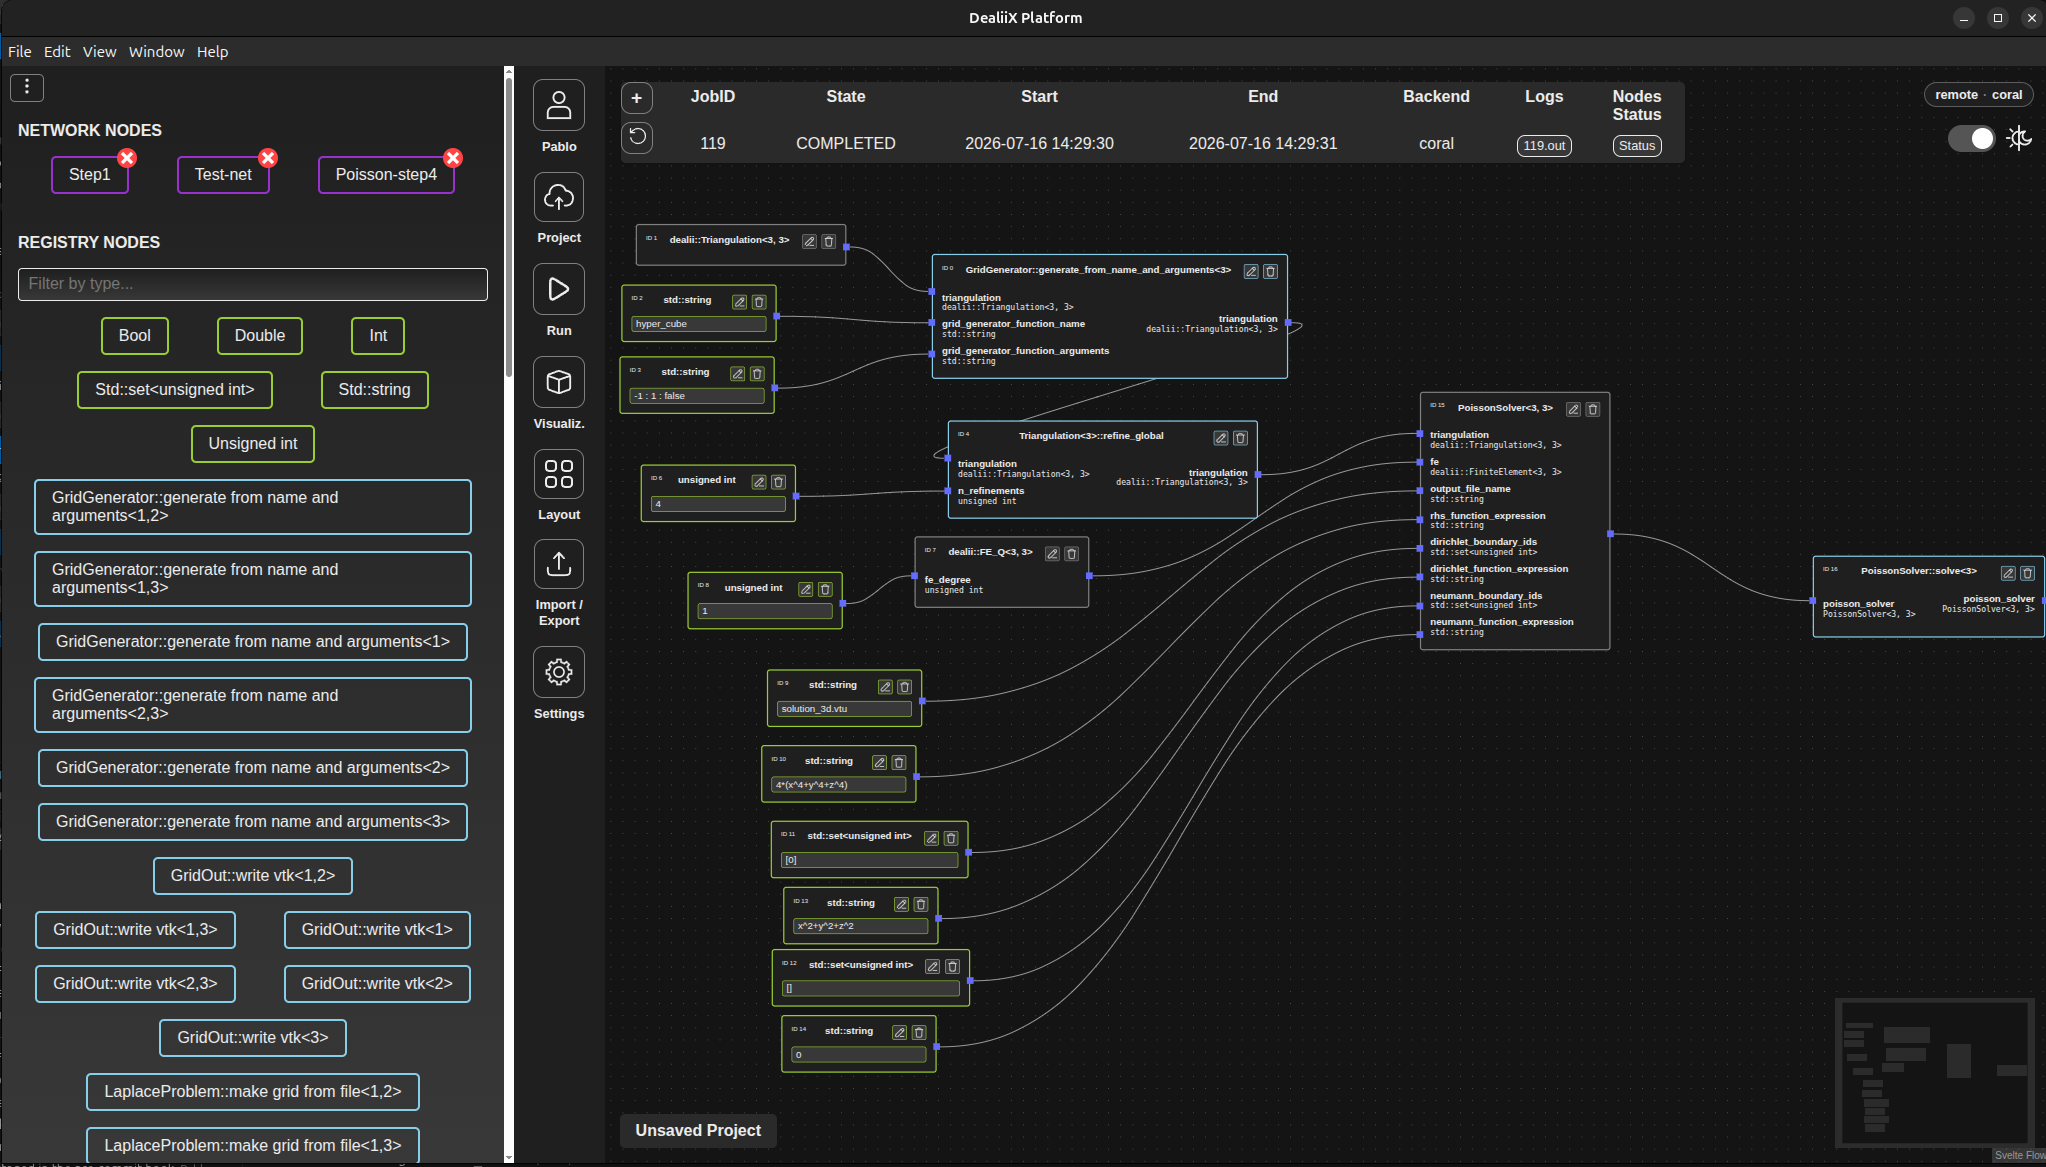
\includegraphics[width=\textwidth]{canvas.png}
    \caption{A computational graph built in the DealiiX Platform's
        node-based low-code editor, executed by CORAL and equivalent to
        deal.II's step-4 tutorial in three dimensions}
    \label{canvas}
\end{figure}

% Keep the figure above the sentence that introduces the feature list, so it
% cannot be placed between that sentence and the list itself.
\FloatBarrier

On top of this typed graph model, the editor (Fig.~\ref{canvas}) provides
the interaction features expected from a modern visual programming
environment:

\begin{itemize}
    \item a searchable node palette, from which nodes are added to the
        canvas via drag and drop;
    \item a create-on-connect flow: dragging a connection onto an empty area
        of the canvas offers the compatible node types and creates the
        selected one, already connected;
    \item editable literal fields directly on primitive nodes, editable node
        names, multi-selection with bulk deletion;
    \item per-level undo/redo history and automatic graph layout based on a
        rank-based algorithm, with horizontal and vertical orientations;
    \item import and export of graphs as JSON files following the network
        protocol, so that graphs can be shared and versioned outside the
        platform;
    \item a light and a dark theme, with a fully semantic color system.
\end{itemize}

Simulation parameters are handled through a dedicated collapsible panel.
The platform \emph{probes} the simulation code to obtain its parameter tree:
following the deal.II parameter handling conventions, both JSON and
\texttt{.prm} text formats are supported, with automatic format detection.
Parameters can be edited, sections can be duplicated (for parameter studies
of repeated subsections), and the resulting file is uploaded alongside the
graph at execution time.

\section{\textcolor{EUblue}{The no-code layer: subnetwork nodes}}

The key feature linking the low-code and the no-code approaches, as
anticipated in D2.6, is the ability to encapsulate a collection of nodes
into a single reusable node. In the deployed platform this is realized by
\emph{subnetwork nodes} (network nodes in the protocol nomenclature).

Any selection of nodes on the canvas can be collapsed into a named
subnetwork node. The platform automatically computes the boundary of the
selection: the unconnected inputs and outputs of the selected nodes become
the external interface of the new node, while the internal edges are hidden.
The resulting node behaves like any other node in the palette --- it can be
dragged onto the canvas, connected, and shared --- but it encapsulates an
entire computational graph, which is stored in its definition following the
network protocol and persisted across sessions.

\begin{figure}
    \centering
    \begin{subfigure}{\textwidth}
        \centering
        \figureOrPlaceholder{subnetwork-collapsed.png}{a subnetwork node
            collapsed on the canvas, exposing only its external interface}
        \caption{a collapsed high-level node}
        \label{subnetwork-a}
    \end{subfigure}

    \vspace{0.6cm}

    \begin{subfigure}{\textwidth}
        \centering
        \figureOrPlaceholder{subnetwork-internal.png}{the internal graph of
            the same subnetwork node, opened for editing, with the breadcrumb
            bar visible}
        \caption{the internal lower-level definition of the subnetwork node
            shown in (\subref{subnetwork-a})}
        \label{subnetwork-b}
    \end{subfigure}
    \caption{Subnetwork nodes}
    \label{subnetwork}
\end{figure}

Subnetworks are fully editable in place: the user can enter a subnetwork
node and modify its internal graph, navigating arbitrarily nested levels
through a breadcrumb bar (Fig.~\ref{subnetwork}). A subnetwork can also be
\emph{exploded} back into its constituent nodes in the parent graph. On
export, every node is annotated with a qualified identifier that encodes its
position in the nesting hierarchy, which is what allows the per-node
execution monitoring described in Sec.~\ref{sec:execution} to work
transparently across nested graphs.

This mechanism directly realizes the vision of D2.6: an expert user builds a
simulation workflow with the low-code editor and collapses it into a single
opaque node --- for example a complete solver that only exposes a mesh input
and a result output --- and a non-expert user then operates purely at the
no-code level, connecting a few high-level nodes and running the simulation
without ever seeing the underlying logic.

% Confine the subnetwork figure to this section.
\FloatBarrier

\section{\textcolor{EUblue}{Execution modes and meta-scheduling}}
\label{sec:execution}

The design requirement of a transparent usage of computational resources is
implemented by a meta-scheduling layer that supports four execution modes,
selected in the application settings and always visible through a dedicated
execution badge:

\begin{itemize}
    \item \textbf{Local + CORAL}: the graph is executed by a CORAL binary
        running directly on the user's machine;
    \item \textbf{Remote + CORAL}: the graph is submitted over SSH to a
        remote system, where it is queued through the Slurm workload manager
        and executed by CORAL;
    \item \textbf{Local + Executable}: any deal.II program following the
        DealiiX executable contract is run locally;
    \item \textbf{Remote + Executable}: the same, on a remote machine over
        SSH.
\end{itemize}

The \emph{executable contract} is a deliberately minimal convention that
makes existing deal.II applications usable from the platform without
modification of the platform itself: when invoked with a parameters file
path that does not exist, the program writes a template file containing all
its parameters and exits (this is the probing step used to build the
parameters panel); when the file exists, the program reads it and runs the
simulation. The standard deal.II tutorial step-70 is included in the
repository as a reference example and works out of the box.

For the remote modes, the platform manages the whole job lifecycle. Graph
and parameter files are uploaded over SSH (using public key authentication),
and a Slurm batch script is generated from a template. Two templates are
provided, for serial and MPI execution; when MPI is enabled, the job
configuration dialog exposes the number of nodes and tasks per node, and the
exported network JSON is annotated with the MPI plugin block required by
CORAL for parallel initialization. Submitted jobs are tracked in a
persistent jobs table (Fig.~\ref{jobs}) showing scheduler status (pending,
running, completed, failed, cancelled), submission and completion times, and
the backend used.
For CORAL jobs, the execution status of every individual node of the graph
--- including nodes nested inside subnetworks, via their qualified
identifiers --- can be inspected from the interface, and the standard output
of the job can be opened directly in the application.

\begin{figure}
    \centering
    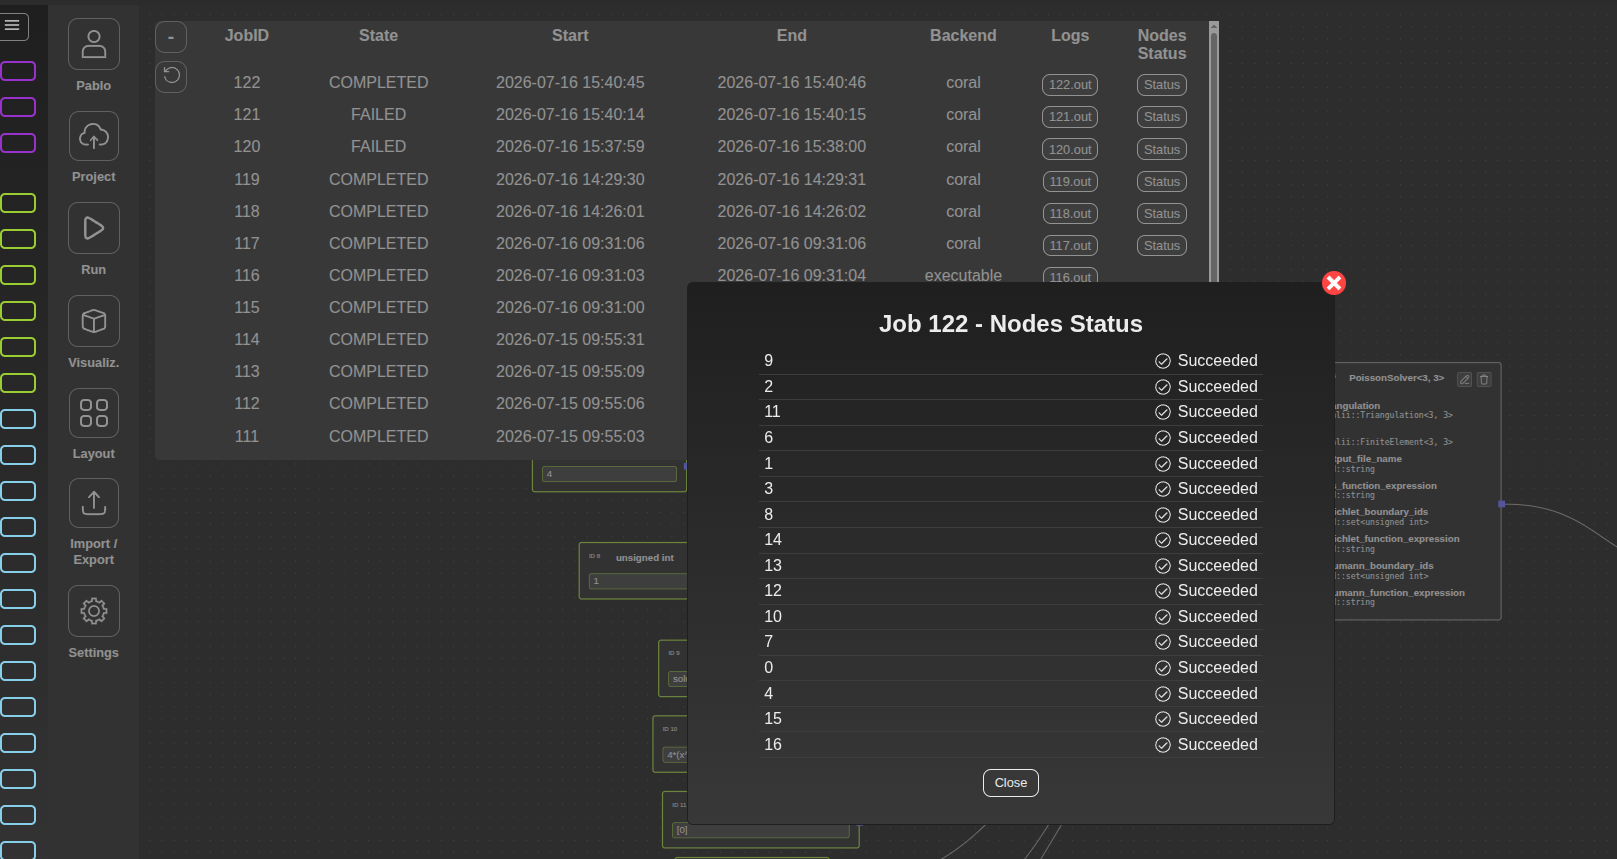
\includegraphics[width=\textwidth]{jobs.png}
    \caption{Job monitoring: jobs table and per-node execution status}
    \label{jobs}
\end{figure}

Two deployment scenarios have been exercised during the testing phase. The
first is a containerized environment, distributed with the platform, in
which a Docker container runs CORAL together with a complete Slurm
installation and an SSH server; this reproduces the interaction with a
remote batch-scheduled cluster faithfully enough to develop and test the
whole submission and monitoring path on a single machine. The second is an
HPC cluster, on which the same containers have been deployed and reached
over SSH, with the procedure documented step by step in the platform
repository:
\url{https://github.com/2listic/dealiiX-platform/blob/main/docs/remote-setup.md}.
Since the platform assumes only SSH access and a Slurm scheduler, the same
mechanism applies to other production HPC systems.

The layer described so far executes a single computational unit (a graph or
an executable) per submission. Its natural extension is the
orchestration of several such units, and this is the purpose of the pipeline
mode described in Sec.~\ref{sec:validation}. At the time of writing the
orchestrator has been designed but not yet developed: the design defines the
pipeline stages, the ordering edges between them and the translation of the
resulting graph into a chain of dependent scheduler jobs, while the
implementation is deliberately left to the final phase of the project, so
that it can be shaped by the feedback of the users who will operate it.

\section{\textcolor{EUblue}{Collaborative and visualization services}}

The collaborative space requirement is served by the Coral Remote Server, a
lightweight REST service with JWT-based authentication. From the
application, users can register and log in, create projects, and save and
load computational graphs to and from the server. Projects can be renamed,
described, deleted, and --- crucially for the collaborative workflows
envisioned in D2.6 --- shared with other users with read or write
permissions. This allows, for instance, an expert user to prepare and share
a validated simulation workflow that a colleague can open and run without
rebuilding it.

\begin{figure}
    \centering
    \figureOrPlaceholder{visualizer-poisson.png}{the Poisson solution
        produced by the graph of Fig.~\ref{canvas}, rendered in the Coral
        Visualizer}
    \caption{Poisson solution in the Coral Visualizer as a result of the
        workflow of Fig.~\ref{canvas}}
    \label{visualizer}
\end{figure}

Simulation results are inspected through the Coral Visualizer
(Fig.~\ref{visualizer}), a web-based viewer for VTK/deal.II output formats
(\texttt{.vtk}, \texttt{.vtu}), reachable directly from the application. During the reporting period the
visualizer has been substantially extended with a ParaView-based rendering
backend providing filters, visualization pipelines, solution field
rendering, cell manipulation and edit sessions, while retaining a
lightweight VTK backend for local usage. The visualizer has been tested with
project-relevant datasets, including vascular geometries such as carotid
artery meshes.

\section{\textcolor{EUblue}{Testing with the lighthouse applications and
early-user feedback}}
\label{sec:validation}

A central goal of the PoC platform is that a user without deep knowledge of
the underlying simulation codes, and without the ability to write deal.II
code or to assemble a computational graph, should still be able to
configure and run a complete simulation. The executable mode described in
Sec.~\ref{sec:execution} realizes this goal directly: given a program that
follows the executable contract, the platform probes it for its parameter
tree, presents that tree in the parameters panel in either JSON or
\texttt{.prm} form, and dispatches the run to the selected local or remote
target through the meta-scheduling layer, with monitoring and output
retrieval available from the same interface. The interaction is reduced to
editing parameters and pressing run.

This path has been tested on two of the dealii-X lighthouse applications,
brain and liver (\texttt{immersx}, elasticity solver), and on the deal.II
tutorial program step-70, which is included in the repository as a reference
example of the contract. Output from these runs was inspected through the
Coral Visualizer; Fig.~\ref{brain} shows results from the brain application.
Because the contract requires no platform-side development per application,
support in executable mode is a property of the mechanism rather than of a
per-application integration effort: the heart (\texttt{lifex},
\texttt{.prm} input) and lungs (\texttt{exadg}, JSON input) applications
comply with the same parameter-file convention and are expected to work
without changes to the platform.

\begin{figure}[!htb]
    \centering
    \figureOrPlaceholder{brain.png}{results of the brain lighthouse
        application rendered in the Coral Visualizer}
    \caption{Results of the brain lighthouse application, inspected in the
        Coral Visualizer}
    \label{brain}
\end{figure}

Testing also showed that the executable mode and the node editor should not
remain two disjoint ways of using the platform. The observation that emerged
most clearly is that an executable is itself a natural unit of composition
(a black box with parameters, a run and an output), and therefore a
natural candidate to become a node. This has led to the design of a
\emph{pipeline mode}, currently under development, in which a higher-level
directed acyclic graph is built whose nodes are entire computational units:
either a complete CORAL graph or a standalone executable. Edges express
execution order, and the resulting graph is topologically sorted and
submitted to the scheduler as a chain of dependent jobs, giving the
meta-scheduler an orchestration capability that neither CORAL nor a single
executable provides on its own. Pipeline mode is a node editor in its own
right, built on the same canvas technology as the low-code editor, and is
therefore positioned to reuse the interaction features already available
there. In this way a lighthouse application driven in executable mode ceases
to be an alternative to the graph paradigm and becomes a component within
it.

Feedback collected from project partners during the testing phase was
consistently positive on the central proposition of D2.6, and converged with
the development team's own findings on the priorities for the final phase,
in particular MPI support in executable mode, the enrichment of the node
registries, and the consolidation of pipeline mode described above, which
originated as a suggestion during this phase.

\FloatBarrier

\section{\textcolor{EUblue}{Packaging, deployment and quality assurance}}

The platform is distributed as native installers for Linux
(\texttt{.deb}) and macOS (\texttt{.dmg}), produced by an automated release
pipeline: tagging a version on the main branch triggers GitHub Actions
workflows that run the full check and test suite, build the application, and
attach the installers to a public GitHub release. For evaluation and
testing, the full server-side stack (CORAL with Slurm and SSH, the remote
server, and the visualizer) is started with a single
\texttt{docker compose up} command.

Six versions have been released during the reporting period, following the
iterative plan of D2.6:

\begin{itemize}
    \item \textbf{1.0.9} (September 2025): first packaged version --- canvas
        editor with typed validation, deal.II nodes, SSH execution;
    \item \textbf{1.1.0} (January 2026): remote server integration
        (authentication, projects, sharing), jobs panel, protocol
        simplification;
    \item \textbf{1.2.0} (January 2026): network (subnetwork) nodes, graph
        download, unit testing infrastructure;
    \item \textbf{1.3.0} (March 2026): MPI support, persistent jobs with
        per-node execution status, job log inspection, parameter handling;
    \item \textbf{1.4.0} (May 2026): execution modes with local runs and the
        executable contract, in-place subnetwork editing, full TypeScript
        migration, redesigned settings;
    \item \textbf{1.4.1} (July 2026): deployment on real remote machines,
        single-command full stack, end-to-end test suites, complete theming
        overhaul, \texttt{.prm} parameter support.
\end{itemize}

Quality assurance is enforced at three levels. At commit time, git hooks run
the linter, the type checker and the code formatter. On every push and pull
request, a continuous integration pipeline runs static type checking of both
the frontend and the Electron backend, plus the unit test suite (Vitest),
and blocks merging on failure. Finally, two tiers of end-to-end tests, based
on Playwright driving the real Electron application, cover the interactive
flows: Tier~1 exercises the canvas (node creation, connections, undo/redo,
graph import, subnetwork collapse and explode) without external services,
and runs headlessly in CI on every push; Tier~2 covers authentication and
project management flows against a live Coral Remote Server instance. Both
tiers run against an isolated configuration store, so tests are reproducible
and cannot interfere with a user's installation.

\section{\textcolor{EUblue}{Outlook}}
\label{sec:outlook}

With the deployment of the first version of the PoC platform, task 2.6.4 of
the development plan presented in D2.6, reproduced in Fig.~\ref{gantt}, is
completed. The
final phase of the project (task 2.6.5, M23--M27) is devoted to the
development of additional features, driven by the feedback collected from
the project partners during the testing period. The main directions are:

\begin{itemize}
    \item enrichment of the node registries with the dealii-X application
        libraries developed in the other work packages, moving from tutorial
        examples towards the organ-scale digital twin workflows targeted by
        the project;
    \item development of the orchestrator designed during this phase: passing
        of artifacts between pipeline stages, verification that the expected
        artifacts of a stage exist before the stages depending on it are
        released, and a short path to edit the parameters of an individual stage of a
        pipeline directly from the orchestrator canvas;
    \item MPI support in executable mode;
    \item continued improvement of the visualization service and of the
        no-code user experience for non-expert users.
\end{itemize}

\begin{figure}
    \centering
    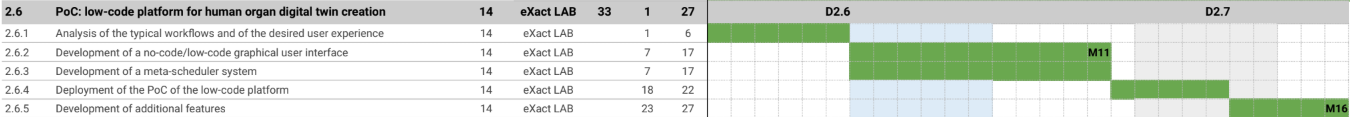
\includegraphics[width=400pt]{gantt.png}
    \caption{Timeline of the activities of task 2.6; D2.7 marks the end of
        the deployment phase (task 2.6.4)}
    \label{gantt}
\end{figure}

The PoC platform is one of the main exploitable results of the dealii-X
project: it demonstrates, end to end, that the simulation capabilities
developed in the project can be operated through an intuitive low-code/no-code
environment by users with widely different technical backgrounds, and it
provides the foundation on which the final version of the platform will be
delivered at the end of the project.

\label{MyLastPage}


\end{document}
